\chapter{Inleiding (les 1)}
\section{Situering}
De cursus situeert zich in het domein: Technisch wetenschappelijk rekenen, in het Engels Scientific Computing/Computational science and engineering.
\\\\
Technologische vraag $\rightarrow$ wiskundig model $\rightarrow$ Numeriek model $\rightarrow$ Algoritme keuze $\rightarrow$ Software implementatie

\begin{description}
	\item [Technologische vraag] wat zijn de krachten die inwerken op een gebouw bij een bepaalde windbelasting, wat is de vervorming van een wagen als hij inrijdt tegen een muur, wat staat er op digitaal ingescand beeld.

	\item [Wiskundig model] een differentiaal vergelijking, groot stelsel, optimalisatieprobleem.

	\item [Numeriek model] wiskundig model in het algemeen niet oplosbaar, van zo een aard dat wiskundige formules inzicht geven maar niet analytisch kan uitgerekend worden, een numeriek model worden opgesteld, een heel groot stelsel.

	\item [Algoritme keuze] gericht op het probleem

	\item [Software implementatie] laat uitvoeren op computer, krijgt veel getallen, aan de hand hiervan probleem oplossen.
\end{description}
Numeriek modellering gaan we in eerste deel van de cursus doen. Hoe van wiskundig model naar numeriek problem. Vaak dingen die geformaliseerd zijn in oneindig dimensionale ruimte, functieruimte. De computer rekent met getallen, dus discretiseren, dan kom je bij de algebra terecht, bij de numerieke modellen (matrices, vectoren). Voor dat numeriek model kiest men een algoritme dit is deel 2 van de cursus.
\\\\
Toepassingen (de wiskunde) die we gaan bekijken:
\begin{itemize}
	\item signaal verwerking
	\item beeld verwerking / restoratie / herkenning / compressie
	\item datamining (scanner beelden vergelijken met databank)
	\item CAD (Computer-aided design)
\end{itemize}

Benaderen algemene aspecten
%\tikzset{
%  nodes around center/.style args={#1:#2:#3:#4}{%
%    at={([shift={(#3)}] {{(\tikzchaincount-1)*360/(#2)+#1}}:{#4})}
%  }
%}
%\begin{tikzpicture}[node distance=5em,every node/.style={circle,draw}]
%  \node [circle] (Z) {Benaderen};
%  \begin{scope}[
%    start chain=circle placed {nodes around center=45:5:Z:10em},
%    every join/.append style={draw=none},
%    every node/.append style={
%      on chain=circle,
%      join,
%      minimum size=5em
%      }
%  ]
%   \node {Waarom};      
%   \node {Hoe};  
%   \node {Criterium};  
%   \node {Waarmee};  
%   \node {Wat discreet};  
%   \chainin (circle-begin);
%  \end{scope}
%\end{tikzpicture}
\tikzset{concept/.append style={fill={none}}}
\begin{figure}[!h]
	\centering
	\begin{tikzpicture}[scale=0.8]
		\path[mindmap,level 1 concept/.append style=
				{sibling angle=72}]
		node[concept,scale=0.7] {\textbf{Benaderen}}
		[clockwise from=90]
		child { node[concept] {Waarom} }
		child { node[concept] {Wat discreet} }
		child { node[concept] {Waarmee} }
		child { node[concept] {Criterium} }
		child { node[concept] {Hoe} };
	\end{tikzpicture}
	\caption{Situering}
	\label{fig:Situering}
\end{figure}

\begin{description}
	\item [Wat] functies continu, discreet 1D/2D/3D
	\item [Waarmee] Veeltermen, trigonometrische functies, splines (veeltermen die aan elkaar vastgangen) basis van tekenprogramma's/tekenfilms, rationale functies, wavelets (compressie in de digitale beeldverwerking, wordt niet besproken in deze cursus), neurale netwerken, support vector machine.
	\item [Criterium] Hoe ga je de kwaliteit van zo een benadering evalueren. Een maatstaf nodig, om te zeggen welk van de 2 benadering beter is (= de kwaliteit van de benadering). Bv kleinste kwadratenbenadering, minimax, Tayler expantie, interpolatie,...
	\item [Hoe]
	\item [Waarom] Compressie beeld, dominante periode te herkennen, beeld restoratie, ruis reductie, parameters in wiskunde model te identificeren.
\end{description}

\subsection{Voorbeeld: benadering van een continue functie}
"Bepaal een veeltermbenadering van graad 4 voor de functie $e^x$ over $[-1,1]$."

\begin{exam} Bespreek het opstellen van een n-de graads Taylor-, interpolatie- en kleinstekwadraten veelterm benadering voor een continue functie f(x) op het interval [a,b]. Hoe stel je de benadering op? Hoe ziet de foutenkromme er uit? Wat zijn de voor- en nadelen van de methodes? Bewijs de stelling over het aantal en de ligging van de nulpunten van de foutenkromme bij de kleinste-kwadratenbenadering. Waarom is de kennis van de nulpunten nuttig? Welk van die methodes zijn bruikbaar voor het benaderen van een discrete functie? Bijvragen: Geef andere voorbeelden van interpolatieveeltermen? (Newton, Vandermonde) Op welke manier wordt de kleinste kwadratenvergelijking opgelost voor continue functies? (Normaalstelsel) Hoe evalueer je de nulpunten van de benaderende fout $r_n = phi_{n+1}(x)$? (Eigenwaarden van tridiagonaalmatrix alpha, nu, lambda)
	\begin{description}
		\item [Taylor-ontwikkeling] in $x=0$ (dus Maclaurin)
		      Functiewaarden in punt 0 alsook van 1 tot 4de orde afgeleide. Onder alle veeltermen is dit de veelterm die het meeste afgeleiden gemeenschappelijk heeft.
		      ${\displaystyle f(x)=f(a)+{\frac {f'(a)}{1!}}(x-a)+{\frac {f''(a)}{2!}}(x-a)^{2}+{\frac {f^{(3)}(a)}{3!}}(x-a)^{3}+\ldots =\sum _{n=0}^{\infty }{\frac {f^{(n)}(a)}{n!}}\,(x-a)^{n}}$

		      ${\displaystyle y_4(x) = 1+x+{\tfrac {1}{2}}x^{2}+{\tfrac {1}{3}}x^{3}+{\tfrac {1}{4}}x^{4} \!}$

		      $ r(s) (residu) = e^x - y_4(x) $

		      Nadeel
		      \begin{itemize}
			      \item  Exact in 0, een fout die heel traag stijgt en het grootst aan de randen, Foutenkromme ongelijkmatig verdeelt, randen $10^-2$ en in center $10^-7$. Liever foutenkromme evenwichtiger.
			      \item Fout kleiner maken door meer termen te nemen, maar dan ben je nog nauwkeuriger in het midden waar je al nauwkeurig genoeg bent.
			      \item Echt veel termen moet meenemen, bij $e^x$ wordt het snel heel klein, elke bijkomende term is veel kleiner als de laatste term, de fout die gemaakt wordt is gelijk aan de eerste term die verwaarloost wordt. Bij $ln(1+x)$ is een Taylor ontwikkeling die heel traag converteert, echt veel termen (termen blijven lang groot) nodig om een bepaalde nauwkeurigheid te bekomen. $ln(1+x) = x - \frac{x^2}{2}+ \frac{x^3}{3}+ \frac{x^4}{4}+ \frac{x^5}{5}$
		      \end{itemize}
		      \begin{figure}[!h]
			      \centering
			      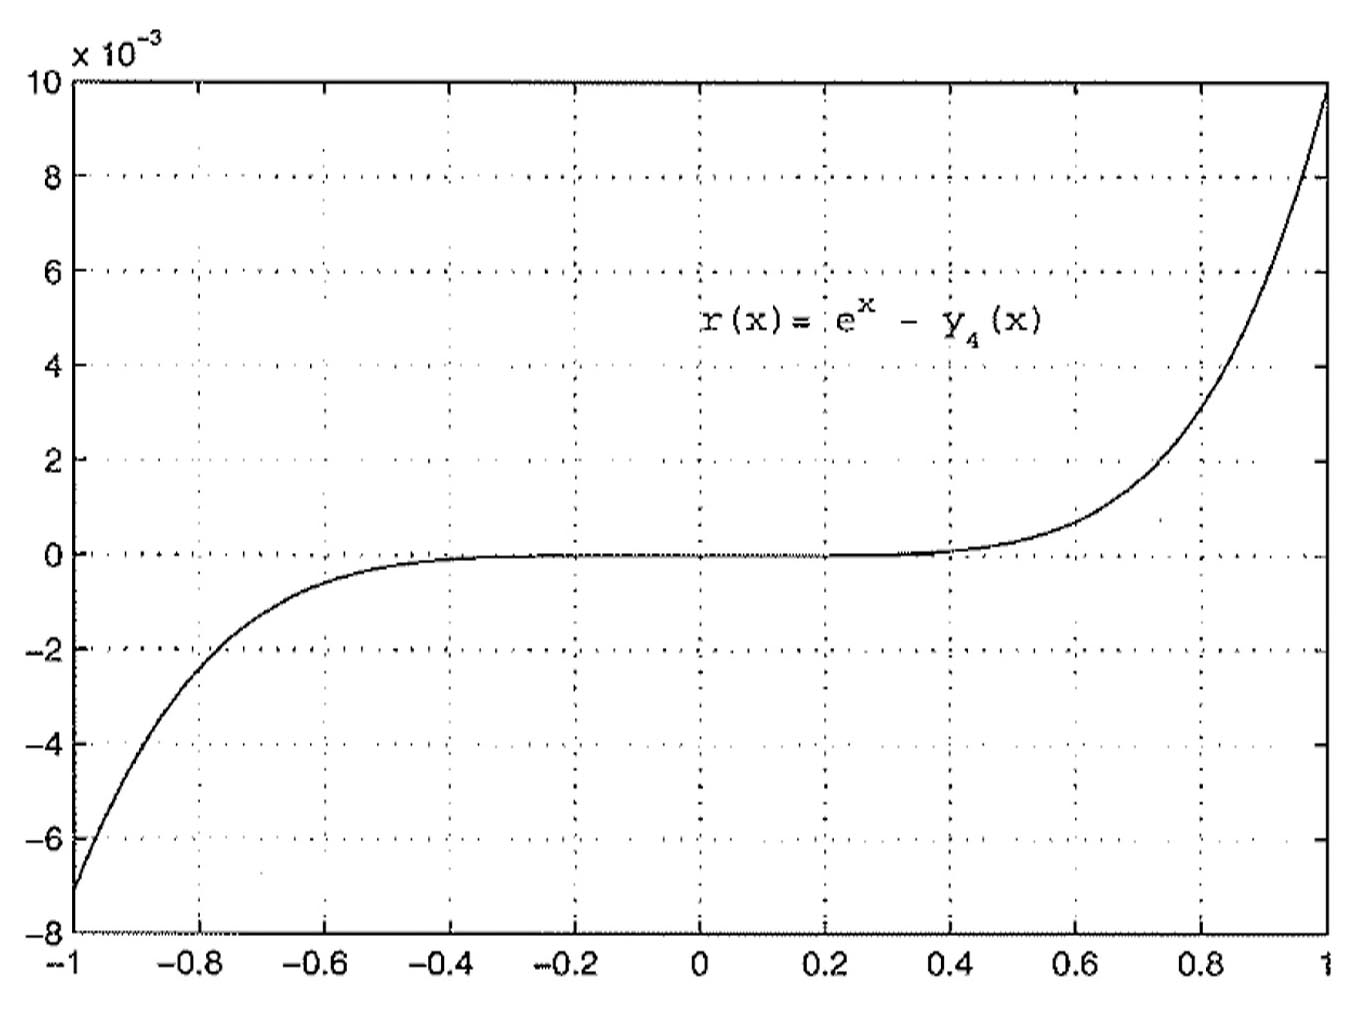
\includegraphics[width=0.5\textwidth]{FoutMaclaurinBenadering}
			      \caption{Fout van de Maclaurin-benadering van graad 4 voor $e^x$}
		      \end{figure}

		\item [Interpolatie] kies een aantal punten, veelterm graad 4 $\rightarrow$ 5 punten nodig van $x_1$ tot $x_5$, mag equidistant liggen of meer geclusterd. Deze punten berekenen op 1 of andere manier (natuurlijk niet met de routine die we nu aan het opstellen zijn), bv Taylor ontwikkeling met 100 termen, veel werk maar niet erg. Belangrijk dat het gebruik heel snel kan.
		      Zodat de veelterm $y_4(x)$ de juiste functiewaarden aanneemt in deze 5 punten (unieke oplossing).
		      Keuze: hoe veeltermen voorstellen? Welk rekenwerk je hebt.
		      Methode:
		      \begin{description}
			      \item [Vandermonde] (monomiale basis) $y_4(x)=a_0+a_1 x+a_2 x^2+a_3 x^3+a_4 x^4$ en eis dat $y_4(x_1) = e^{x_1} ,  y_4(x_2) = e^{x_2},y_4(x_3) = e^{x_3},y_4(x_4) = e^{x_4},y_4(x_5) = e^{x_5}$  $\rightarrow$ stelsel \\ Matrix:
			            ${\begin{bmatrix}1&x_{0}&x_{0}^{2}&\ldots &x_{0}^{n}\\1&x_{1}&x_{1}^{2}&\ldots &x_{1}^{n}\\\vdots &\vdots &\vdots &&\vdots \\1&x_{n}&x_{n}^{2}&\ldots &x_{n}^{n}\\\end{bmatrix}}{\begin{bmatrix}a_{0}\\a_{1}\\\vdots \\a_{n}\end{bmatrix}}={\begin{bmatrix}y_{0}\\y_{1}\\\vdots \\y_{n}\end{bmatrix}}.$
			      \item [Newton]  $y_4(x)=a_0+a_1(x-x_1)+a_2(x-x_1)(x-x_2)+a_3(x-x_1)(x-x_2)(x-x_3)+a_4(x-x_1)(x-x_2)(x-x_3)(x-x_4)$
			            Voordeel $a_k$ zonder stelsel op te lossen, via gedeelde differenties.
			      \item [Lagrange]  \begin{form}
				            $y_4(x):=\sum _{k=1}^{5}e^{xk}l_k(x)$
			            \end{form}
			            Geeft een expliciete oplossing, geen rekenwerk meer. Gemakkelijk op te stellen moeilijk te evalueren. Veelterm wordt geschreven als een lineaire combinatie van de functiewaarden $e^{xk}$ (gekende getallen) met de basisfuncties (functies veelterm van graad 4 zodat $l_i(x_j)$ = 0 indien i $i \neq j$ en 1 indien $i=j$
			            \\
			            \begin{form}
				            $l_k(x)={\frac {(x-x_{0})}{(x_{k}-x_{0})}}\cdots {\frac {(x-x_{k-1})}{(x_{k}-x_{k-1})}}{\frac {(x-x_{k+1})}{(x_{k}-x_{k+1})}}\cdots {\frac {(x-x_{N})}{(x_{k}-x_{N})}}$
			            \end{form}
		      \end{description}
		      $ r(s) (residu) = e^x - y_4(x) $
		      Residu 0 in de meetpunten. Punten wat verschuiven verandert de foutencurve. Foutencurve overal even groot.
		      Nadeel, moeilijk om de punten te selecteren. Waar kies je de punten? Functie ergens lokaal vreemde vorm? Wat als we hier geen punten zetten, dan mist men deze vorm. Nog een nadeel opstellen zorgt voor afrondingsfouten. Veeltermco\"effici\"enten gevoelig voor afrondingsfouten.

		      \begin{figure}[h]
			      \centering
			      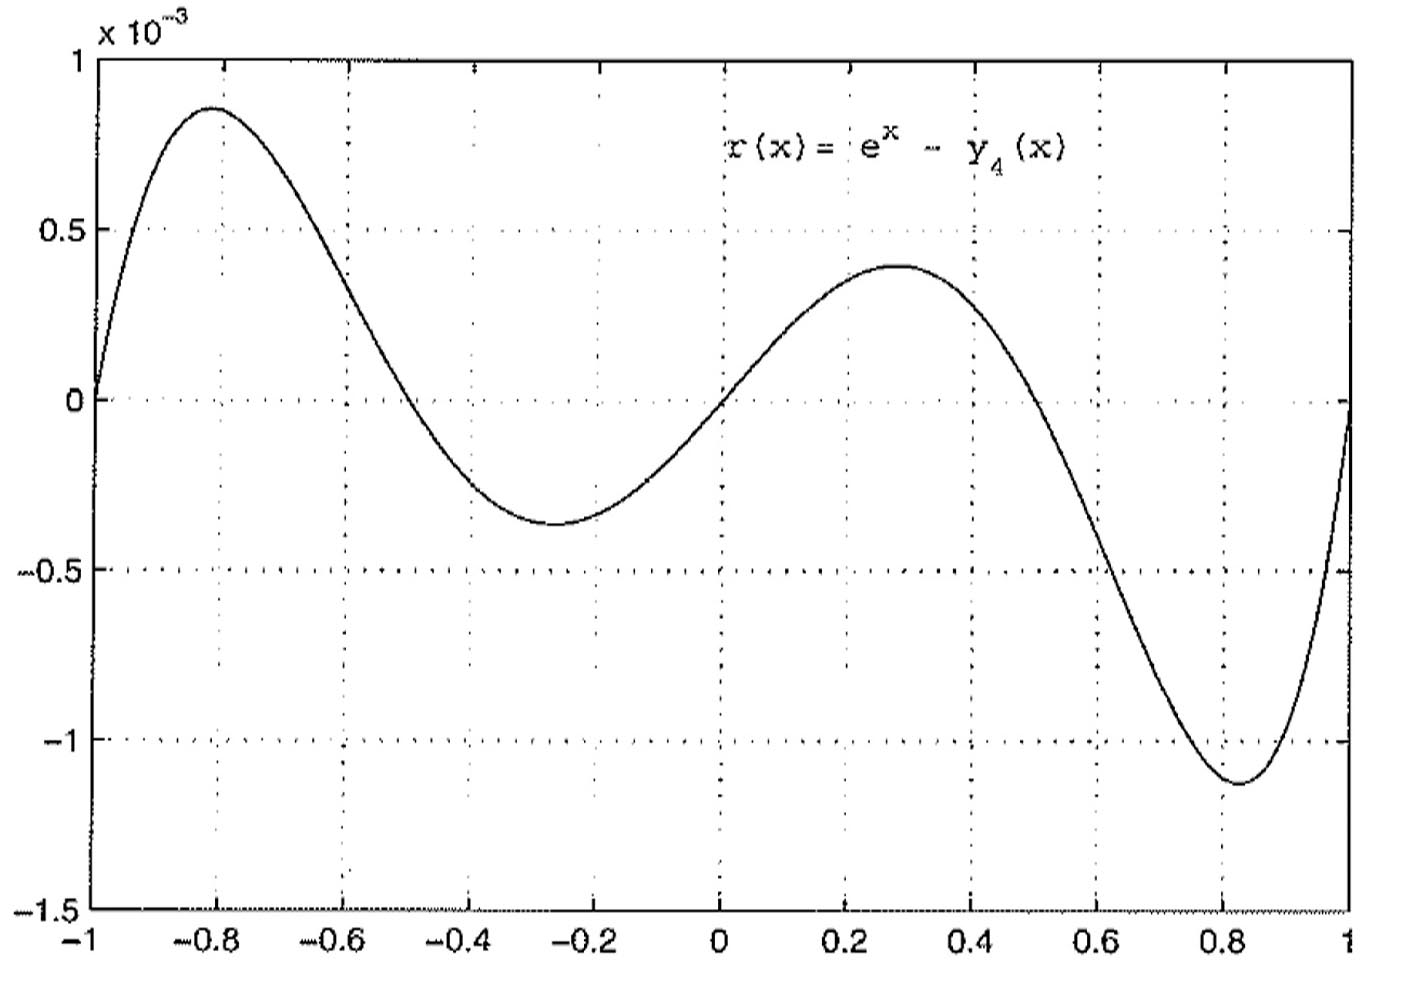
\includegraphics[width=0.5\textwidth]{FoutInterpolerendeBenadering}
			      \caption{Fout van een interpolerende benadering van graad 4 voor $e^x$}
		      \end{figure}

		\item [Minimax] verschil met vorige, hier houdt men rekening met volledige functie/interval, waardoor we geen lokale pieken/singulariteiten missen.
		      $y_4(x) = \underset{y_4\in P_4[-1,1]}{\operatorname {arg\,min}}\underset{x\in [-1;1]}{\operatorname {max}}|e^x - y_4(x)|$
		      Veelterm van graad 4, 5 co\"effici\"enten, element van 5 dimensionale ruimte, zoek maximum in absolute waarde in interval $[-1;1]$, is een getal dat we willen minimaliseren, zoek minimum in de verzameling van alle veeltermen van $y_4$ die behoren tot de ruimte van de veelterm die gaat van $[-1;1]$. De gezochte veelterm is waar het maximum geminimaliseerd wordt. Is een optimalisatiecriterium in een 5 dimensionale ruimte.

		\item [Kleinste kwadraten] Ook een optimalisatie probleem, maar nu afwijking tussen benadering en de te benaderen functie anders formuleren. Verschil met mini max, nu wel makkelijk uit te rekenen
		      $y_4(x) = \underset{y_4\in P_4[-1,1]}{\operatorname {arg\,min}} \int_{-1}^1 w(x) (e^x-y_4(x))^2 dx $

		      Keuze $w(x)$ geeft aan waar je fout liefst kleinst wilt hebben, gewichtsfunctie \\
		      $w(x) \equiv 1 \rightarrow$ legendre \\
		      $w(x) = \frac{1}{\sqrt{1-x}} \rightarrow $ chebyshev, randen oneindig veel gewicht
		      \begin{figure}[h]
			      \centering
			      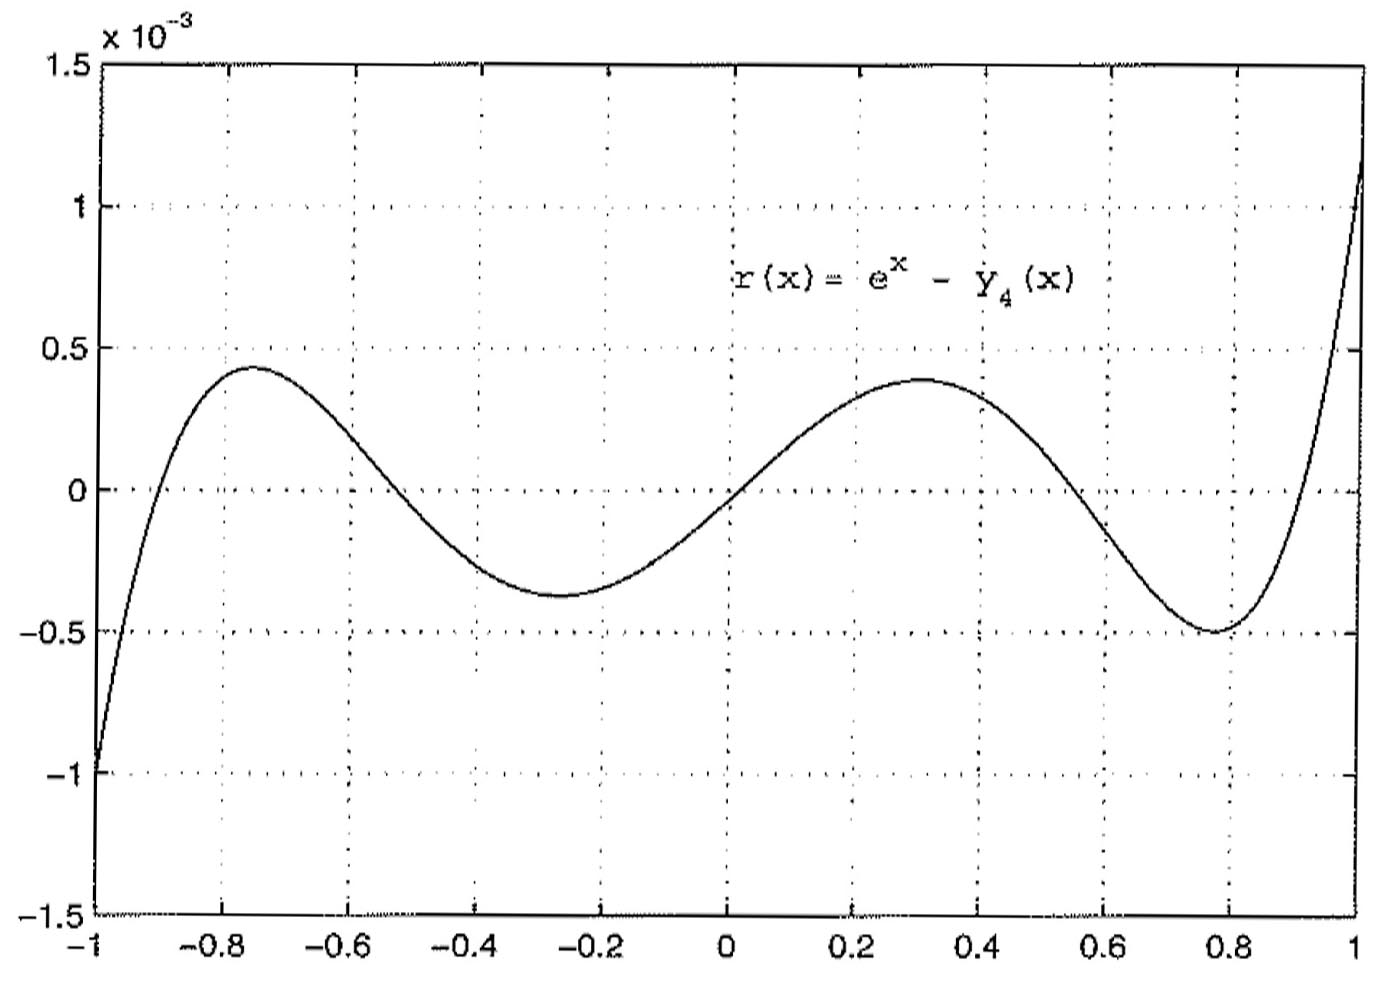
\includegraphics[width=0.5\textwidth]{FoutKleinsteKwadratenLegenreBenadering}
			      \caption{Fout van een kleinste-kwadraten benadering van graad 4 voor $e^x$ met $w(x)\equiv 1$}
		      \end{figure}
		      \begin{figure}[h]
			      \centering
			      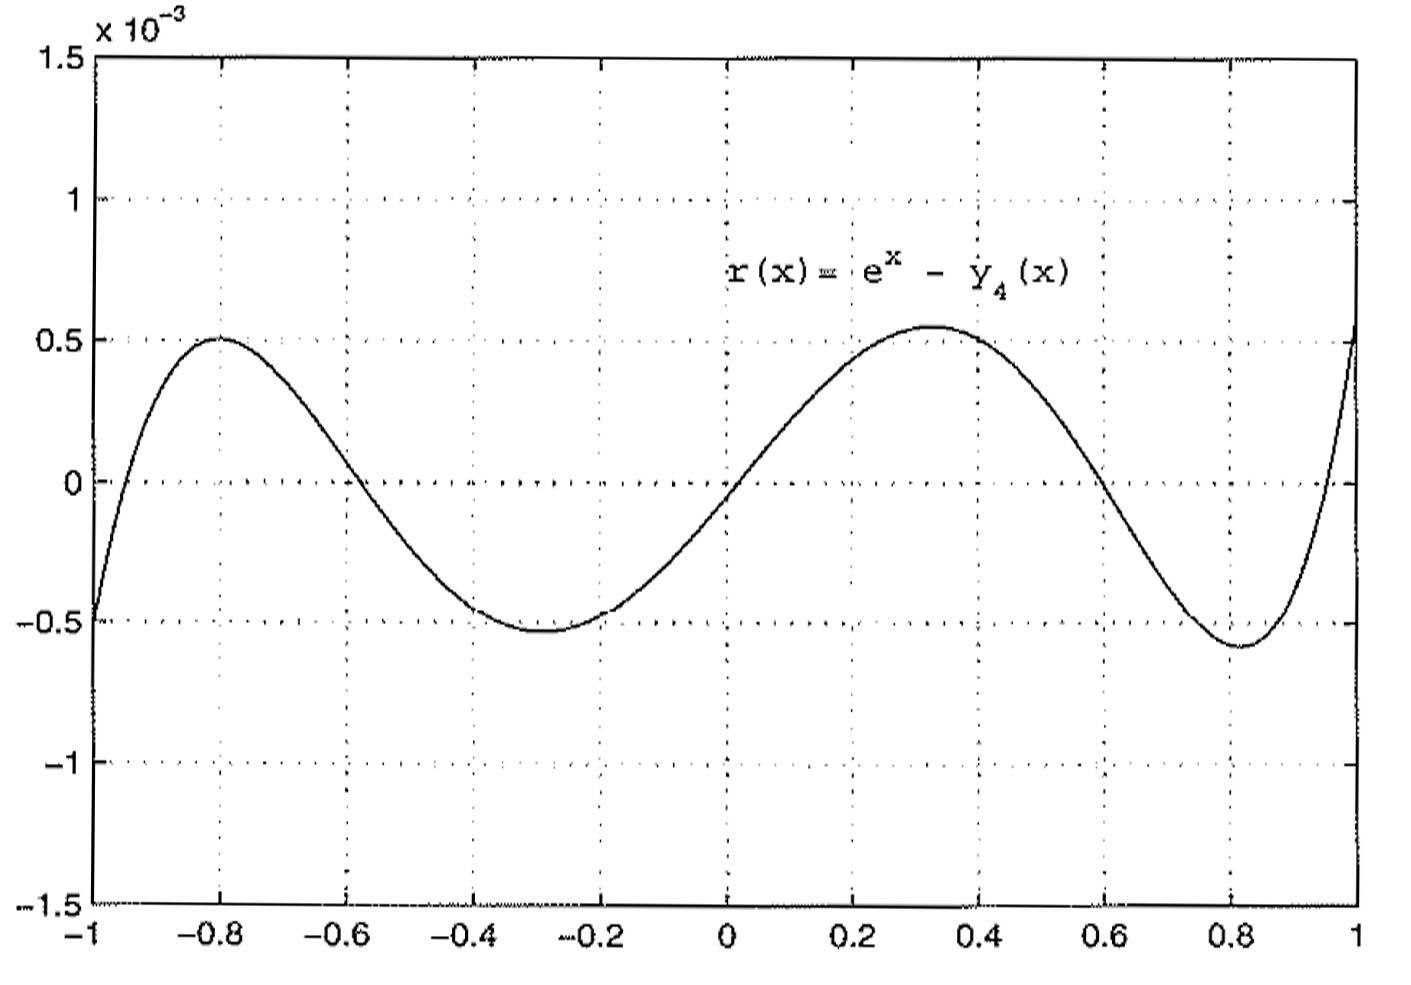
\includegraphics[width=0.5\textwidth]{FoutKleinsteKwadratenChebyshevBenadering}
			      \caption{Fout van een kleinste-kwadraten benadering van graad 4 voor $e^x$ met $w(x)=\frac{1}{\sqrt{1-x}}$}
		      \end{figure}
	\end{description}

	\subsection{Voorbeeld: benaderen discrete functie}
	Zoek een veelterm die goed aansluit bij de dingen je opgemeten hebt.
	\begin{description}
		\item[Taylor-ontwikkeling] NIET Afgeleide nodig, van continue functie hier niet
		\item[Interpolatie] NIET Geen reden om exact door de punten te gaan. Of als je miljoen punten hebt dan benadering van veelterm graad miljoen, niet te evalueren. Welke punten selecteren en hoeveel?
		\item[Minimax]  $y_n(x) = \underset{y\in P_n}{\operatorname {arg\,min}}\underset{i=1,\ldots,N}{\operatorname {max}}|f_i - y(x_i)|$
		      Als meetwaarden vrij nauwkeurig is, anders vermenigvuldigen met $\frac{1}{meetfout}$
		\item[Kleinste kwadraten]
		      $y_4(x) = \underset{y\in P_n }{\operatorname {arg\,min}} \sum_{-1}^1 w(x) (f_i-y(x))^2 dx $
	\end{description}
\end{exam}

\subsection{Keuze benaderingsfuncties}
Waarmee ga je benaderen? Veelterm niet altijd geschikt, altijd oneindig links en rechts dan komt ie naar de oorsprong schommelt een paar keer en dan naar oneindig. Niet alles wat we willen benaderen heeft deze vorm.
Onze (lineaire) benadering zal altijd combinatie zijn van gekende functies en de co\"effici\"enten.
$y(x)=\sum_{k=0} a_k \phi_k(n)$ waar $ \phi_k(n)$ gekend is.
\\\\
Waarom andere basissen:
\begin{itemize}
	\item eenvoud
	\item vorm
	\item fysische toepassing
	\item numeriek, nauwkeurigheid (afrondingsfouten, conditiegetal bij veeltermen, zeker bij monomiale basis zeer slecht)
\end{itemize}